\documentclass[12pt]{book}

%These tell TeX which packages to use.
\usepackage{array,epsfig}
\usepackage{amsmath}
\usepackage{amsfonts}
\usepackage{amssymb}
\usepackage{amsxtra}
\usepackage{amsthm}
\usepackage{mathrsfs}
\usepackage{color}
\usepackage{eurosym}
\usepackage{times}
%Here I define some theorem styles and shortcut commands for symbols I use often
\theoremstyle{definition}
\newtheorem{defn}{Definition}
\newtheorem{thm}{Theorem}
\newtheorem{cor}{Corollary}
\newtheorem*{rmk}{Remark}
\newtheorem{lem}{Lemma}
\newtheorem*{joke}{Joke}
\newtheorem{ex}{Example}
\newtheorem*{soln}{Solution}
\newtheorem{prop}{Proposition}

\newcommand{\lra}{\longrightarrow}
\newcommand{\ra}{\rightarrow}
\newcommand{\surj}{\twoheadrightarrow}
\newcommand{\graph}{\mathrm{graph}}
\newcommand{\bb}[1]{\mathbb{#1}}
\newcommand{\Z}{\bb{Z}}
\newcommand{\Q}{\bb{Q}}
\newcommand{\R}{\bb{R}}
\newcommand{\C}{\bb{C}}
\newcommand{\N}{\bb{N}}
\newcommand{\M}{\mathbf{M}}
\newcommand{\m}{\mathbf{m}}
\newcommand{\MM}{\mathscr{M}}
\newcommand{\HH}{\mathscr{H}}
\newcommand{\Om}{\Omega}
\newcommand{\Ho}{\in\HH(\Om)}
\newcommand{\bd}{\partial}
\newcommand{\del}{\partial}
\newcommand{\bardel}{\overline\partial}
\newcommand{\textdf}[1]{\textbf{\textsf{#1}}\index{#1}}
\newcommand{\img}{\mathrm{omega}}
\newcommand{\ip}[2]{\left\langle{#1},{#2}\right\rangle}
\newcommand{\inter}[1]{\mathrm{int}{#1}}
\newcommand{\exter}[1]{\mathrm{ext}{#1}}
\newcommand{\cl}[1]{\mathrm{cl}{#1}}
\newcommand{\ds}{\displaystyle}
\newcommand{\vol}{\mathrm{vol}}
\newcommand{\cnt}{\mathrm{ct}}
\newcommand{\osc}{\mathrm{osc}}
\newcommand{\LL}{\mathbf{L}}
\newcommand{\UU}{\mathbf{U}}
\newcommand{\support}{\mathrm{support}}
\newcommand{\AND}{\;\wedge\;}
\newcommand{\OR}{\;\vee\;}
\newcommand{\Oset}{\varnothing}
\newcommand{\st}{\ni}
\newcommand{\wh}{\widehat}

%Pagination stuff.
\setlength{\topmargin}{-.3 in}
\setlength{\oddsidemargin}{0in}
\setlength{\evensidemargin}{0in}
\setlength{\textheight}{9.in}
\setlength{\textwidth}{6.5in}
\pagestyle{empty}

\begin{document}

\begin{center}
{\Large DATA 221 \\  Homework 4  \textbf{(rev 0)}}\\
\textbf{Trimble/Nussbaum}\\ %You should put your name here
Due: Monday 2022-02-06  - 11:59pm
\end{center}

\vspace{0.2 cm}

Let's look at the MNIST database of handwritten digits.  The data are two sets of 60,000 images (28x28 pixel handwritten digits, encoded as 8-bit greyscale images / 1x784 element vectors.)

To get started, you will need to flatten the images into 1-dimensional vectors and put the class labels into one-hot encoding.

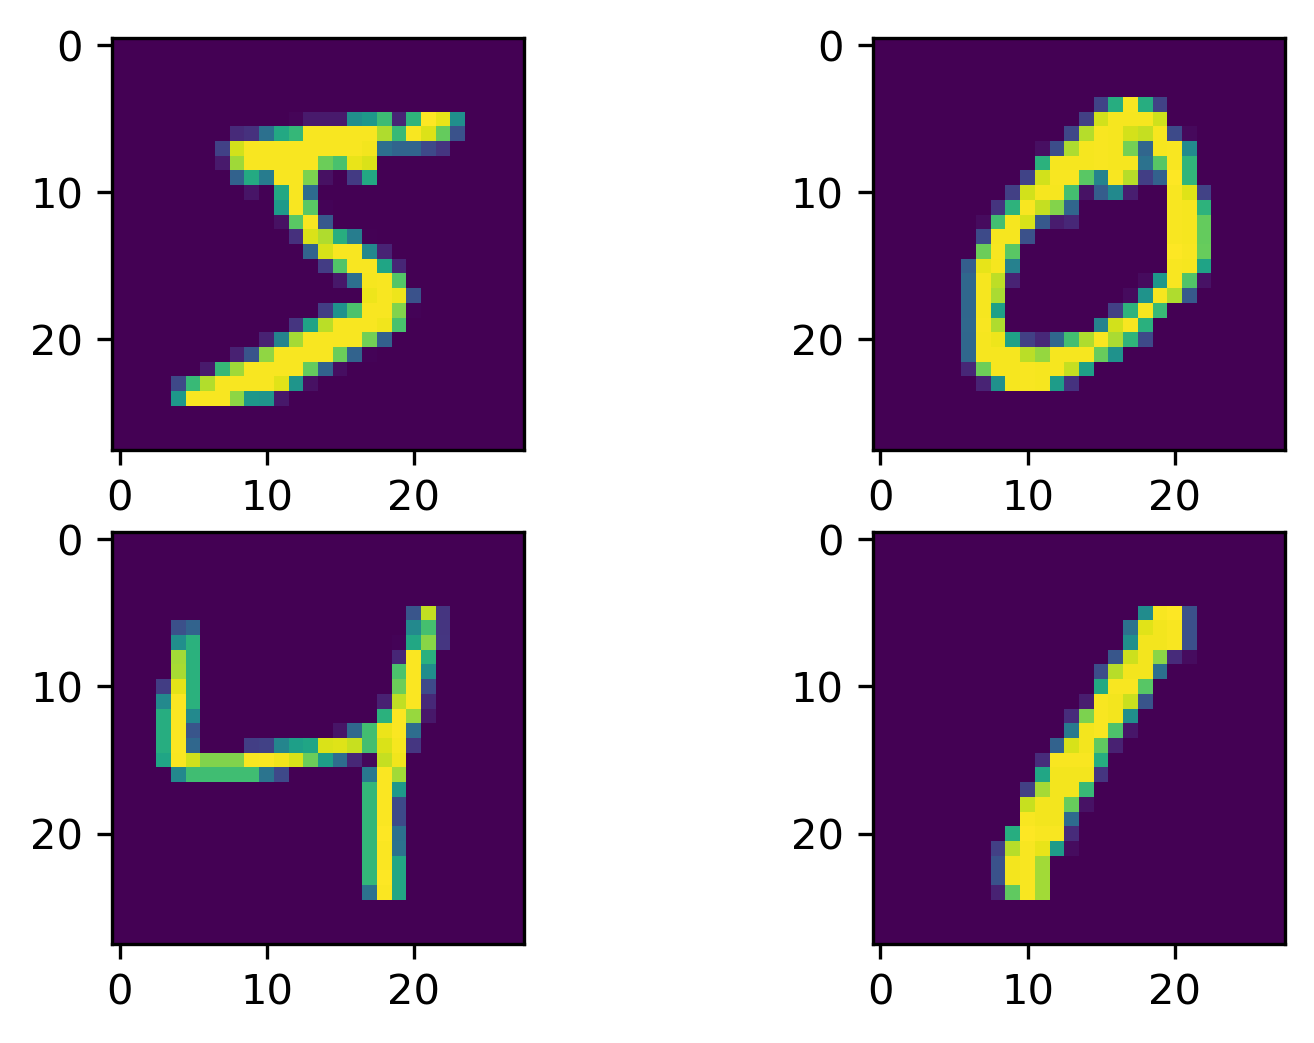
\includegraphics[width=2.3in]{src/MNIST.png}

\begin{enumerate}

\item
Train a neural network with 0 hidden layers on the 60,000 MNIST training images.  The 0-hidden-layer neural network can be thought of as logistic regression or the single-layer perceptron.
Classify the test set and report the confusion matrix for the classifier.

\item
Train a neural network with 1 hidden layers on the MNIST training images.  Report the confusion matrix on the test set.

\item
Train a neural network with more than 1 hidden layer on the MNIST training images.  Report the confusion matrix on the test set.

\item
Some pairs of digits are more easily confused than others.  Choose at least three cells in the confusion matrix and display at least three images of digits that were confused in particular ways,  say, 5 is misclassified as 3.   Which digit pair is hardest to discern?  

% 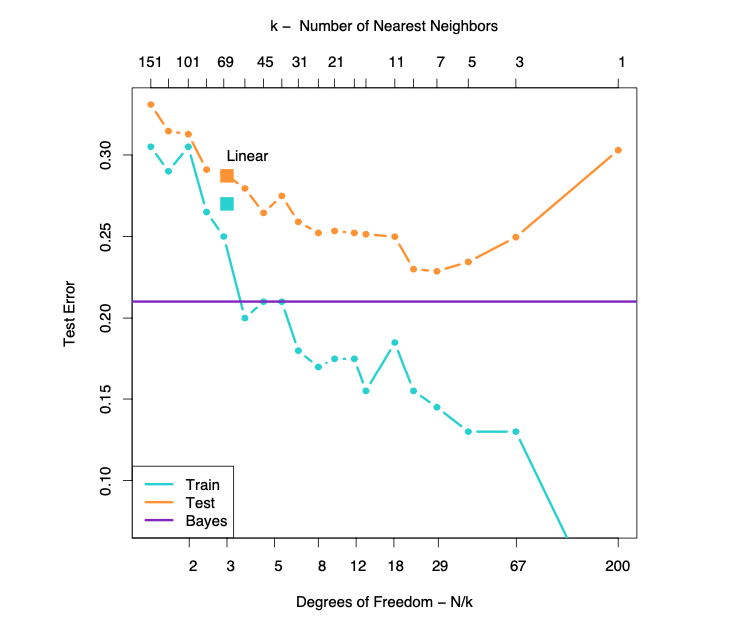
\includegraphics[width=4in]{hastie-generalization.png}
\item 
The first layer of the model can be interpreted as weights-per-pixel; it can be interpreted as a linear inner product filter on the input.   
Take a handful (perhaps 9 or 16) columns from the first-layer weights and display them as images.  Are the input weights for the 4-layer model qualitatively different from the input weights for the 1-layer model?
Hint:  This is an example from the sklearn documentation:

\texttt{https://scikit-learn.org/stable/auto\_examples/neural\_networks/ \
plot\_mnist\_filters.html}

\end{enumerate}
\end{document}


